% !TEX root =  paper.tex

\section{Background and Motivating Example}
\Cref{fig:acc-testing-motivating-example} shows an example of
an inaccessible web page. 
In a quick glance at the rendered page in \Cref{fig:acc-testing-motivating-example}-(c),
a sighted user can immediately understand
the structure of the page and navigate their way through
the various contents of the page.
For instance, the user would immediately recognize 
that they can navigate to other areas of the web site 
through the navigation menu at the top 
(i.e., Home, News, FAQ). 

While this happens naturally and instantaneously for sighted users, 
that is not the case for non-sighted users. 
The page structure (e.g., the presence of a navigation bar at the top)
is \emph{communicated exclusively} through visual design, 
since the HTML markup in \Cref{fig:acc-testing-motivating-example}(a) 
is simply a collection of \code{<div>}s that do not communicate  
any semantic functionality. 
This implicit visual communication is intuitive and natural 
for sighted developers and users, but is unavailable 
for users who can not have \emph{access} to visual 
information due to disabilities. 
Accordingly, the markup is deemed \emph{inaccessible}, 
because it is expressed in a fashion that does not provide 
any semantic information about the page structure.  

\begin{figure*}%[h]
	\centering
    \noindent
    \begin{minipage}[c]{.4\textwidth}
        \centering
        \begin{lstlisting}[language={html},frame=ltbr,
            aboveskip=1.0em]
  <div class="nv8471">
  <div>Home</div>
  <div>News</div>
  <div>FAQ</div>
  <div>Contact</div>
  </div>
        
  <div class="_hd902">
  Resources
  </div>
  <div>
   ...
  </div>
  
  <div class="_hd902">
  About Us
  </div>
  <div>
   ...
  </div>
        \end{lstlisting}
    	(a) HTML markup
    \end{minipage}
%    \hfill
\  \  \  \  \  \ 
    \begin{minipage}[c]{.45\textwidth}
        \centering
        \begin{lstlisting}[language={CSS},frame=ltbr,
            aboveskip=1.0em]
.nav8471 {
   background-color:
    #ffff00;
   display:
    flex;
   justify-content:
    space-around;
   font-weight:
    bold;
   border:
    2px solid #000000;
}
._hd902 {
   font-size:
    5vw;
   font-weight:
    900;
   padding:
    8vh 0 2vh 0;
}
        \end{lstlisting}
    	(b) CSS declaration
    \end{minipage}
%    \hfill
    \begin{minipage}[c]{.85\textwidth}
        \centering
        \ \\ \ \\ 
        \fbox{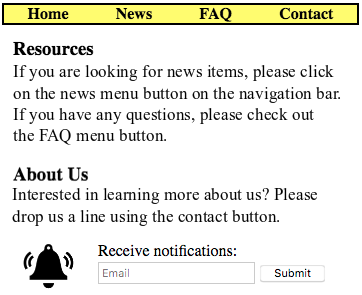
\includegraphics[scale=0.5]{accessibility_testing/figures/motivating-example/rendered-3.png}}
        \\ (c) Rendered page
    \end{minipage}
  
%    \begin{minipage}[c]{.6\columnwidth}\centering
%        (a) HTML code
%    \end{minipage}
%    \hfill
%    \begin{minipage}[c]{.5\columnwidth}\centering
%        (b) CSS declaration
%    \end{minipage}
%    \hfill    
%    \begin{minipage}[c]{.85\columnwidth}\centering
%        (c) Rendered page
%    \end{minipage}    
    \ \\ \caption{An example of an inaccessible web page.}
    \label{fig:acc-testing-motivating-example}
  \end{figure*}

The analysis and conclusion that we just made is currently 
being done manually, since it requires high level semantic analysis of the page. 
Our goal in this work is to automate the reasoning we have 
just described in order to be able to automatically 
reach conclusions about the accessibility of web pages. 


\subsection{ARIA  Roles}\label{subsec:aria-roles}
The aforementioned lack of semantic markup in the 
code makes it difficult for non-sighted 
users to navigate the page. This is because such users rely on 
\emph{screen readers} to parse the page for them 
and present them with the various information or navigation options present in the page. 
Screen readers are tools that speak out the various options, regions, or tasks accessible 
from the page, and the non-sighted user would then select one of the options they heard from 
the screen reader. 
Screen readers can be thought of as web browsers for non-sighted users, 
with one major caveat.
While a standard web browser simply renders the page as is and leaves 
it to the end user to understand what the various elements mean, 
screen readers expect that the page markup contains semantic information 
about various areas of the page, which the reader would then announce audibly, 
giving non-sighted users an understanding of the overall semantic structure of the page.

The standard that is used by screen readers during their processing of 
web pages is the W3C \emph{Accessible Rich Internet Applications} 
(ARIA)~\cite{ARIA} semantic markup.
The ARIA standard specifies a set of markup attributes that 
should be included in the page's HTML to make it accessible to screen readers 
or other assistive technologies. An example of such ARIA attributes is presented in the following subsection. 

\header{Targeted roles}\label{header:targeted-roles}
ARIA defines more than 80 attributes spanning various aspects of the page, 
from low level syntax requirements to high level semantic structure. 
We therefore have to target a subset of these ARIA attributes because 
addressing all 80+ attributes in a single academic work is untractable. 
The basis for selecting the targeted roles is that we focus on the most 
commonly used subset of ARIA, which are \emph{landmark roles}~\cite{2019users_survey}.  
Our own experimental results (\Cref{subsec:run-results}) also demonstrate the 
widespread use of these roles.
The roles identify the major high-level regions of the page and 
specify the semantic role for each of them.  
They consist of a set of specific pre-defined roles that convey, 
though markup, the otherwise only visually perceived role of each region.
For instance, the yellow rectangle at the top of \Cref{fig:motivating-example}(c) 
is perceivable as being a navigation bar, 
therefore the markup of the element containing that region has 
to include the landmark attribute \code{role="navigation"}. 
When a non-sighted user loads the page, the screen reader would read out loud (i.e., generated audible speech) the presence of a navigation bar (and any other semantic regions in the page), allowing the user to quickly perceive the high level structure of the page, and directly interact with the region they are looking for.

Accordingly, the absence of semantic markup in \Cref{fig:motivating-example}(a) 
makes the page inaccessible, because screen readers would be unable to 
provide alternative, non-visual, means of accessing the page.  
That is, the information and cues about the
structure and navigation of the page remain locked 
in the visual design of the page and can not be 
accessed non-visually.
When a web page communicates the important and key aspects of its structure and function using only visual design, without providing a programmatic means to access the same information, it is deemed inaccessible.

\subsection{Existing Tools: Syntax  Checkers}\label{subsec:syncheckers}
Existing accessibility testing tools~\cite{ukgov:audit:2018} are 
based on syntactic checking. 
They check the HTML against certain syntax rules. 
For instance, one common check is to assert that every \code{img} element 
has an \code{alt} text attribute (for text descriptions). 
Another check asserts that \code{input} elements must not 
be descendent of \code{a}.
Another example is checking that every \code{form} 
element has a \code{label} attribute.  
 
While such syntax checks can be useful simple 
assertions and are easy to automate, 
none of the existing tools perform the more important, 
and more challenging, high level \emph{semantic} 
analysis of the page's content. 
For instance, consider the subfigure (c) in \Cref{fig:motivating-example}, 
where we can see that there is a navigation bar at the top. 
Now consider the HTML in subfigure (a), where we observe that 
the developer did not use the required ARIA attribute 
of \code{role="navigation"}. 
Accordingly, because we visually see a navigation region in (c) 
but do not find it expressed in the markup in (a), 
we conclude that the page has an accessibility failure, 
because we perceived a certain semantic structure as sighted users, 
but it was not expressed in the markup in order to ensure it would 
be equally available for non-sighted users. 
That is the the \emph{central} issue in accessibility: 
making sure that whatever is visually perceived 
is also expressed in the code. 

We now pause to reflect and observe that there is no syntactic check 
that can automate the conclusion we just reached. 
That is, the process that we just walked through requires 
our own visual perception as humans in order to reach the conclusion 
that there is a mismatch between the perceived page and the markup. 
This process cannot be expressed in the form of a syntax check. 

In the next section, we describe how we construct an approach that automates the accessibility testing procedure that we have just manually conducted. 